\input ../setup

\usepackage{hyperref}
\usepackage{listings}
\usepackage{color}
\usepackage{enumerate}
\usepackage{graphicx}
\usepackage{tikz-qtree}
\usepackage{amsmath}
\usepackage{amssymb}

% \renewcommand{\labelenumi}{\alph{enumi}.}
% \renewcommand{\labelenumii}{(\roman{enumii})}

\definecolor{mygreen}{rgb}{0,0.6,0}
\definecolor{mygray}{rgb}{0.5,0.5,0.5}
\definecolor{mymauve}{rgb}{0.58,0,0.82}


\lstdefinestyle{normalPy}{
language=Python,				% the language of the code
basicstyle=\footnotesize,			% the size of the fonts that are used for the code
numbers=left,				% where to put the line-numbers; possible values are (none, left, right)
numberstyle=\color{mygray},		% the style that is used for the line-numbers
stepnumber=1,				% the step between two line-numbers. If it's 1, each line will be numbered
numbersep=5pt,				% how far the line-numbers are from the code
backgroundcolor=\color{white},		% choose the background color; you must add \usepackage{color} or \usepackage{xcolor}
showstringspaces=false,			% underline spaces within strings only
showspaces=false,				% show spaces everywhere adding particular underscores; it overrides 'showstringspaces'
showtabs=false,				% show tabs within strings adding particular underscores
frame=shadowbox,				% adds a frame around the code
tabsize=4,					% sets default tabsize to 4 spaces
captionpos=t,				% sets the caption-position to bottom
breaklines=true,				% sets automatic line breaking
breakatwhitespace=false,			% sets if automatic breaks should only happen at whitespace
commentstyle=\color{mygreen},    	% comment style
keepspaces=true,                 		% keeps spaces in text, useful for keeping indentation of code (possibly needs columns=flexible)
keywordstyle=\color{blue},       		% keyword style
}

\lstdefinestyle{consolePy}{
stepnumber=0,
}
\tikzset{every tree node/.style={minimum width=2em,draw,circle},
         blank/.style={draw=none},
         edge from parent/.style=
         {draw, edge from parent path={(\tikzparentnode) -- (\tikzchildnode)}},
         level distance=1.5cm}

\begin{document}
%%%%%%%%%%%%%%%%%%%%%%%%%%%%%%%%%%%%%%%%%%%%%%%
\psetheader{Extra Practice 7}{}
%%%%%%%%%%%%%%%%%%%%%%%%%%%%%%%%%%%%%%%%%%%%%%%

\medskip

For Questions 1-3, you can choose any data structure to use for each question!
\section{Question 1}
We are given a certain amount of money and we are allowed to buy any 2 things in a
supermarket. We are only allowed to spend the exact amount of money we are given
(i.e. the 2 things we choose to buy must add up exactly to the amount we were given).
Given a list containing the prices of all the items in the supermarket, define a function
\texttt{\bfseries find\_positions} that takes in the list of prices, and the amount of money we have,
and returns a tuple containing the two indexes, i and j, such that the list at indexes i and
j both add up to the amount we have. Take note that $i \neq j$. \\ \\
You can assume that there is only one correct answer (if any). If there is no possible
answer, return 0. \\ \\
\textbf{Sample Tests:}
\begin{python}
>>> find_positions([4, 2, 1, 8, 5], 3)
(1, 2)  # 2+1=3
>>> find_positions([4, 2, 1, 8, 5], 5)
(0, 2)  # 4+1=5
>>> find_positions([4, 2, 1, 8, 5], 8)
0       # must be 2 items added up
>>> find_positions([4, 2, 1, 8, 5], 12)
(0, 3)  # 4+8=12
\end{python}
\textbf{Note: What is the time and space complexity of your solution? Can you do better?}

\section{Question 2}
In the supermarket, there are n rows of m items in each row. Each item has a price
on it. Assume that you are at the supermarket with your girlfiend (or boyfriend) who has a habit of
buying everything you walk past. Given that you are at the start of the supermarket (row
1 column 1) and want to exit the supermarket located at row n column m, you wish to move in a
path such that you can minimize the total amount that you need to spend. Define a
function, \texttt{\bfseries cheapest\_path} that takes in a matrix and returns the least amount of
money you can possibly spend. (Note: You can only move downwards or rightwards)
\newpage
\textbf{Sample Test:}
\begin{python}
>>> matrix = [[3,3,1],
              [2,9,4],
              [7,2,1],
              [1,5,2]]
>>> cheapest_path(matrix)
14
\end{python}
\textbf{Note: How does our code change if we now want to start from the bottom left
corner, move either upwards or rightwards until we reach the top right corner?}

\section{Question 3}
Two words are considered to be \textit{isomorphic} if each letter in one word can be mapped
over to another letter. For instance, the words "aba" and "dad" are isomorphic where the
letter "a" can be mapped over to "d", and the letter "b" can be mapped over to "a". In
contrast, "deeds" and "poopp" are not considered isomorphic because more than one
letter ("d" and "s") maps to the same letter "p". "deeds" and "poops" are isomorphic
because "d" $\rightarrow$ "p", "e" $\rightarrow$ "o", "s" $\rightarrow$ "s". \\ \\
Define a function \texttt{\bfseries check} that takes in two words as inputs and returns \texttt{\bfseries True} if both
words are isomorphic to each other, and \texttt{\bfseries False} otherwise. \\ \\
\textbf{Sample Test:}
\begin{python}
>>> check("aba", "dad")
True
>>> check("aba", "dae")
False
>>> check("aba", "bab")
True
>>> check("deeds", "poops")
True
>>> check("deeds", "poopp")
False
\end{python}

\newpage

\section{Question 4 (WARNING: Challenging!)}
\textbf{\textit{(CS1010X AY16/17 Special Term I Finals, abridged)}} \\ \\
In this problem, we will work with recursive lists of a special form where the last element points
to the next list and the last list in the series points back to the first list in the series. Each list is
also called a \textit{link} (of the chain). This is illustrated here:
\begin{center}
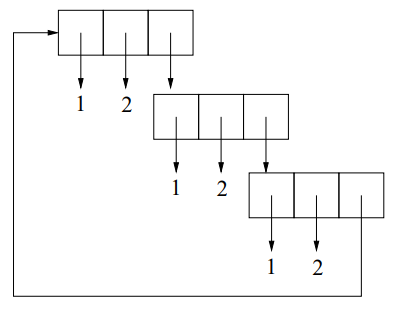
\includegraphics[scale=0.9]{chain.png}
\end{center}
\begin{enumerate}[(a)]
\item The function \texttt{\bfseries chain(seq, n)} creates a chain of $n$ links by replicating a 
sequence \texttt{\bfseries seq} as follows:
\begin{python}
>>> chain((1, 2), 1)
[1, 2, [...]]
>>> chain((1, 2), 3) # Illustrated above
[1, 2, [1, 2, [1, 2, [...]]]]
>>> chain((4,), 4)
[4, [4, [4, [4, [...]]]]]
\end{python}
Give a possible implementation for \texttt{\bfseries chain(seq, n)}.

\item Given a chain it would certainly be helpful to be able to count the number of links in the
chain. For example:
\begin{python}
>>> count_links(chain((1, 2), 1))
1
>>> count_links(chain([3, 2], 2))
2
>>> count_links(chain((4,), 4))
4
\end{python}
Give a possible implementation for \texttt{\bfseries count\_links}.

\item A regular chain has repeated links. It is possible for a fault to happen and one of the links
might become "faulty". A faulty link has one element that is different from all the other links.
Implement the function \texttt{\bfseries find\_fault} that will return the different element. You can assume that
the chain has at least 3 links and there’s only one faulty element.
\begin{python}
>>> a = chain((1, 2), 4)
>>> a[2][2][0] = 5
>>> a
[1, 2, [1, 2, [5, 2, [1, 2, [...]]]]]
>>> find_fault(a)
5
\end{python}
\end{enumerate}
\end{document}